%% chapter 4 dataset, network structure, experiment and result
\chapter{实验与结果}
\label{cha:experiment}
我们在实验中采用滚动步态作为仿真爬杆实验的基本步态,为了验证蛇形机器人在我们提出的自适应控制框架下能够对于变化的环境表现出适应性,我们在V-REP(Virtual Robotics Experimentation Platform)机器人仿真实验平台上进行建模实验,让机器人在我们的控制框架下在不同直径的杆进行自适应地攀爬运动。

仿真实验主要分为两个过程:训练和运动仿真。我们将运动仿真实验分为两组实验,分别是沿着直径变化的杆的自适应运动实验以及沿着不同直径的直杆做自适应运动实验。
\section{训练过程}
\begin{figure}[!h]
	\centering
	\includegraphics[width=0.9\linewidth,height=0.35\textheight]{figure/chap05/clusize.eps}
	\caption{K-MEANS++中不同$N_{k}$取值时的簇方差}
	\label{fig:clusize}
\end{figure}
在数据获取阶段,我们让蛇形机器人在不同的多组参数组合下在25\,cm 和 35\,cm的杆上进行无目的性的攀爬运动,最终总共我们能收集到2万5千组的训练数据。控制参数幅度$A$,相位$\varepsilon$ 和角速度$\omega$的变化区间分别为$[40, \, 80]$,$[0, \, 5]$以及$[1.5, \, 3]$。并且, 幅度参数$A$的变化步长是5,相位参数$\varepsilon$的变化步长是1,以及角速度参数的变化步长为$\omega$ 0.5。 我们让蛇形机器人在不同参数组合下进行爬杆运动,在爬杆过程中收集相应的数据。在数据预处理阶段,我们对训练数据做一个聚类操作。我们通过算式\ref{clu_var}求出不同$N_{k}$的取值下的簇方差(如图\ref{fig:clusize})。最终$N_{k}=25$下的K-MEANS++聚类结果如图\ref{fig:clustersize},可以看到大多数簇的成员数量为$1000 \pm 500 $。

\begin{figure}[t]
	\centering
	\includegraphics[width=0.6\linewidth]{figure/chap05/cluster.eps}
	\caption{$N_{k}=25$时使用K-MEANS++聚类的结果}
	\label{fig:clustersize}
\end{figure}

\section{机器人在直径可变杆上的运动实验}
在这一部分仿真实验中,我们的实验环境是一个复杂的杆模型。实验所用杆模型主要分为三个部分。 第一和第三部分,即最低和最高的部分的杆的直径都为35\,cm,中间部分用直径为25\,cm的杆来连接。 我们在蛇形机器人80s的运动中记录下记录参数和速度的变化。

记录下来的实验结果如图\ref{fig:BSB}所示。在0\,s到4\,蛇形机器人在初始参数下是无法蜷缩到能卷紧杆的状态的,所以机器人在一开始会不断调整自己的形状以卷紧未知直径的杆。所以在这一阶段,Z轴速度的值是接近于0的。从24\,s到45\,s的运动中,蛇形机器人在直径为 35\,cm的杆上进行攀爬运动。在这一阶段,控制参数$A$, $\varepsilon$以及$\omega$全部都在改变并且 $A$和 $\varepsilon$ 最终会趋于一个比较稳定的值。大概在45\,s时,蛇形机器人到达了杆的直径发生变化的节点,由于直径变化的幅度很大,所以机器人无法马上去卷紧下一个不同直径的杆,于是便导致了这里Z轴速度会接近于0。通过我们提出的运动控制框架,蛇形机器人可以自动调整参数来适应下一个不同直径的杆来继续其攀爬运动。 从图\ref{fig:bsa}, \ref{fig:bsp} 和 \ref{fig:bsw}可以得到,在这个变杆节点参数都在变大,从而顺利地让蛇形机器人可以继续往上爬。同样地,在大概 63\,s时,蛇形机器人来到了第二个变杆节点。蛇形机器人此时也是自动调整控制参数来顺利地继续往上爬。然后可以看到最终所有参数都会趋于一个稳定的值,原因也是后面杆的直径没有再发生变化从而不需要再去调整步态参数来对突变环境做适应性运动。
\begin{figure}[htbp]
	\centering
	\begin{subfigure}{0.3\textwidth}{
			\centering
			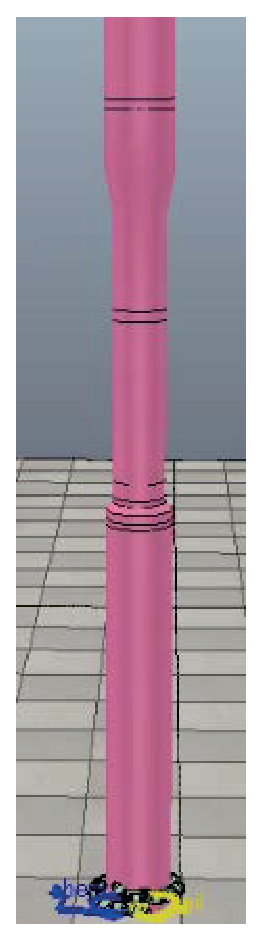
\includegraphics[height=160pt,width=0.5\textwidth]{figure/chap05/BSB/34s.eps}
			\caption{t=24s}
		}
	\end{subfigure}
	\begin{subfigure}{0.3\textwidth}{
			\centering
			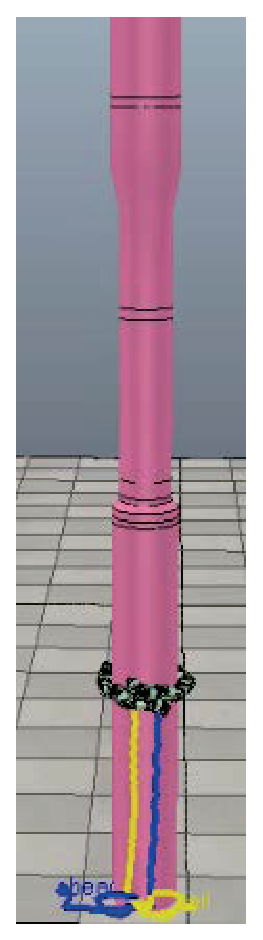
\includegraphics[height=160pt,width=0.5\textwidth]{figure/chap05/BSB/49s.eps}
			\caption{t=35s}
		}
	\end{subfigure}
	\begin{subfigure}{0.3\textwidth}{
			\centering
			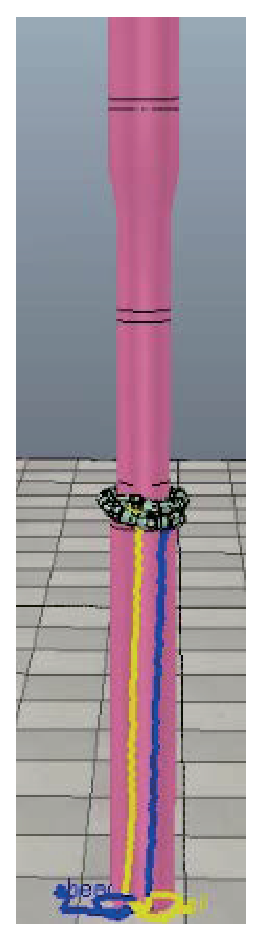
\includegraphics[height=160pt,width=0.5\textwidth]{figure/chap05/BSB/1m05s.eps}
			\caption{t=47s}
		}
	\end{subfigure}
	\begin{subfigure}{0.3\textwidth}{
			\centering
			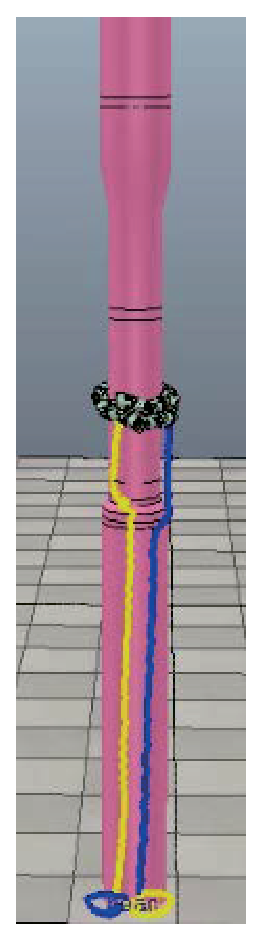
\includegraphics[height=160pt,width=0.5\textwidth]{figure/chap05/BSB/1m17s.eps}
			\caption{t=56s}
		}
	\end{subfigure}
	\begin{subfigure}{0.3\textwidth}{
			\centering
			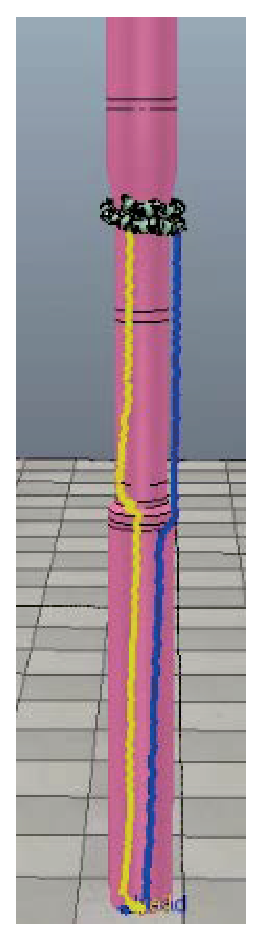
\includegraphics[height=160pt,width=0.5\textwidth]{figure/chap05/BSB/1m27s.eps}
			\caption{t=63s}
		}
	\end{subfigure}
	\begin{subfigure}{0.3\textwidth}{
			\centering
			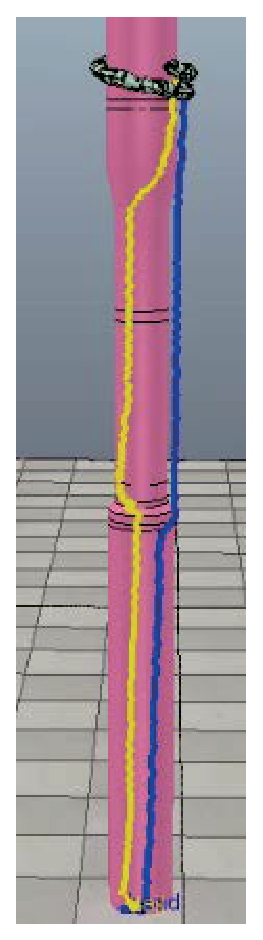
\includegraphics[height=160pt,width=0.5\textwidth]{figure/chap05/BSB/1m35s.eps}
			\caption{t=69s}
		}
	\end{subfigure}
	\begin{subfigure}{0.45\textwidth}{
			\centering
			\includegraphics[width=1\textwidth,height=130pt]{figure/chap05/BSB/a.eps}
			\caption{幅度参数$A$随时间的变化}
			\label{fig:bsa}
		}
	\end{subfigure}
	\begin{subfigure}{0.45\textwidth}{
			\centering
			\includegraphics[width=1\textwidth,height=130pt]{figure/chap05/BSB/p.eps}
			\caption{相位参数$\varepsilon$随时间的变化}
			\label{fig:bsp}
		}
	\end{subfigure}
	\begin{subfigure}{0.45\textwidth}{
			\centering
			\includegraphics[width=1\textwidth,height=130pt]{figure/chap05/BSB/w.eps}
			\caption{角速度参数$\omega$随时间的变化}
			\label{fig:bsw}
		}
	\end{subfigure}
	\begin{subfigure}{0.45\textwidth}{
			\centering
			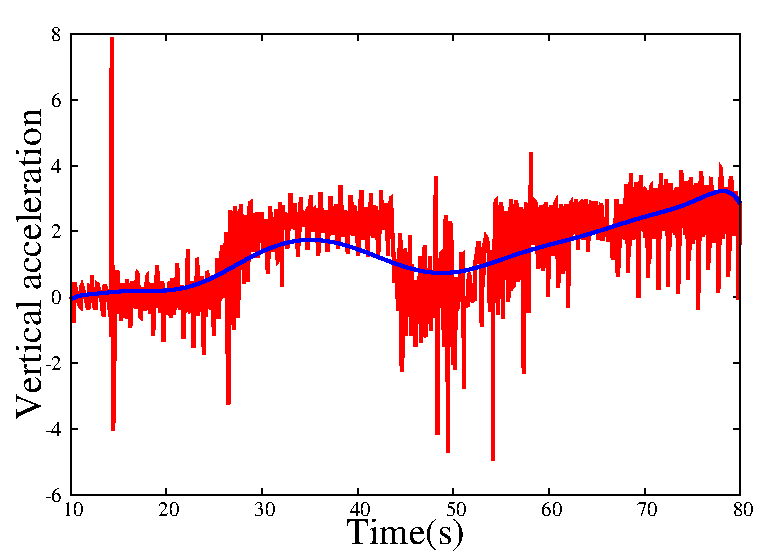
\includegraphics[width=1\textwidth,height=130pt]{figure/chap05/BSB/v}
			\caption{Z轴速度随时间的变化}
			\label{fig:bsv}
		}
	\end{subfigure}
	\caption{图(a)到(f)描述了蛇形机器人的攀爬过程。图(g)到(j) 是控制参数和Z轴速度在运动过程中的的变化曲线。}
	\label{fig:BSB}
\end{figure}


最终,所有控制参数包括Z轴速度也是趋近于一个稳定的值。说明了我们的控制策略可以让蛇形机器人去自动调整自身的运动来适应变化的运动环境。

实验证明了我们的控制策略对于机器人在直径可变杆做适应性自主运动是行之有效的。


\section{在不同直径杆上的运动对比实验}

由于现实世界中的环境是未知且复杂多变的,训练所用的环境和现实环境可能存在差异。我们训练环境为直径为25\,cm和35\,cm的直杆。为了验证我们的控制策略能够用于实际的多样化的场景,我们在直径为 20\,cm,,25\,cm, 30\,cm,35\,cm和40\,cm的杆上进行了独立的验证实验。实验结果如图\ref{fig:scurve}。

\begin{figure}[htbp]
	\centering
	\begin{subfigure}{0.45\textwidth}{
			\centering
			\includegraphics[width=1\textwidth,height=130pt]{figure/chap05/samplifier.eps}
			\caption{幅度参数$A$随时间的变化}
			\label{fig:samplifier}
		}
	\end{subfigure}
	\begin{subfigure}{0.45\textwidth}{
			\centering
			\includegraphics[width=1\textwidth,height=130pt]{figure/chap05/sphase.eps}
			\caption{相位参数$\varepsilon$随时间的变化}
			\label{fig:sphase}
		}
	\end{subfigure}
	\begin{subfigure}{0.45\textwidth}{
			\centering
			\includegraphics[width=1\textwidth,height=130pt]{figure/chap05/sarate.eps}	
			\caption{角速度参数$\omega$随时间的变化}
			\label{fig:sarate}
		}
	\end{subfigure}
	\begin{subfigure}{0.45\textwidth}{
			\centering
			\includegraphics[width=1\textwidth,height=130pt]{figure/chap05/svel.eps}
			\caption{Z轴速度随时间的变化}
			\label{fig:svelocity}
		}
	\end{subfigure}
	\caption{蛇形机器人在不同直径的杆上运动的参数及速度曲线图}
	\label{fig:scurve}
\end{figure}

接下来对实验结果进行详细地分析。通过观察参数变化曲线,我们可以得出杆的直径越小,对于蛇形机器人来说需要更多的时间去从初始步态来调整到合适的步态,原因是初始步态是统一的。对于直径为40\,cm的杆的实验场景,由于蛇形机器人关节数的限制,无法形成一个首尾相接的环来环抱40\,cm的杆。在这种情况下,由于不需要去形成螺旋状的步态,所以相位参数$\varepsilon$的作用就会变得十分弱图\ref{fig:sphase}。因此对于直径更小的杆,例如直径为20\,cm的杆,只调整幅度参数$A$是不足以让机器人能够很好地环抱杆从而保证顺利攀爬。因此,在直径更小的杆下进行攀爬运动,蛇形机器人会不断调整相位参数$\varepsilon$配合幅度参数$A$的调整来使得步态,机器人形状很好地支撑攀爬运动(图\ref{fig:samplifier},\ref{fig:sphase})。实验结果表明,我们的控制策略能够帮助蛇形机器人能够在未知的直径的杆上不断调整自身步态来进行攀爬且最终都达到了一个合适且稳定的步态。

在所有实验环境中,机器人的运动速度最终会围绕一个值上下波动(图\ref{fig:svelocity})。杆的直径的变化仅仅影响速度曲线的收敛速度,即机器人达到稳定速度的耗时。机器人运动的步态控制参数最终也是会收敛达到稳定(图\ref{fig:scurve})。这表明了外部环境的变化对控制策略的影响非常微弱。最终机器人将在其运动过程中能够不断找到最需要调整的参数并且进行计算调整。



\section{算法效率}
图\ref{fig:CE-TS}描述了我们的控制策略中算法的计算开销以及蛇形机器人在不同直径的杆上进行攀爬运动的耗时统计。

\begin{figure}[htbp]
	\centering
	\begin{subfigure}{0.45\textwidth}{
		\centering
		\includegraphics[width=1\textwidth,height=140pt]{figure/chap05/figCE.eps}
		\label{fig:CE}
		\caption{攀爬运动时算法的每一次计算耗时}
	}
	\end{subfigure}
	\begin{subfigure}{0.45\textwidth}{
		\centering
		\includegraphics[width=1\textwidth,height=140pt]{figure/chap05/TimeSpent.eps}
		\label{fig:TS}
		\caption{攀爬运动的耗时}
	}
	\end{subfigure}
	\caption{蛇形机器人在5米高的不同直径的杆时的算法的最差,最佳以及平均计算耗时和攀爬运动总时长}
	\label{fig:CE-TS}
\end{figure}

我们可以看到,无论杆的直径如何,算法的计算耗时都是相似的,这表明我们的控制策略的算法计算开销不仅在一个可忽略的范围内,而且受环境的影响也很小。 可以观察到机器人会花费更多时间来攀爬直径较小的杆。 原因是蛇形机器人需要更多的时间将初始步态调整为合适的步态。

实验结果表明,通过我们提出的控制策略可以实现蛇形机器人运动中的自适应控制。



